% \documentclass[runningheads,a4paper]{llncs}
% \usepackage[final]{nogamacro}
% \usepackage[driverfallback=dvipdfm]{hyperref}
% \usepackage[final]{nogaref}
% \usepackage{amsmath}
% \usepackage{cite}
% \usepackage{amssymb}
% \setcounter{tocdepth}{3}
% \usepackage{graphicx}
% \usepackage{url}
% \usepackage{bibnames}
% \usepackage{multirow}
% \usepackage{booktabs,caption,fixltx2e}
% \usepackage[flushleft]{threeparttable}
% \usepackage[misc,geometry]{ifsym}
% \usepackage{bbding_mod}

%To show no page number and stop runnig heads
% \pagestyle{empty}

% \newcommand{\keywords}[1]{\par\addvspace\baselineskip
% \noindent\keywordname\enspace\ignorespaces#1}



% \begin{document}

% \mainmatter  % start of an individual contribution

% % first the title is needed
% \title{Efficient Scalar Multiplication for Ate Based Pairing over KSS Curve of Embedding Degree 18}

% % suggested  running head
% \titlerunning{Efficient SCM for Ate-based Pairing over KSS Curve}
% % the name(s) of the author(s) follow(s) next

% \author{Md. Al-Amin Khandaker\inst{1 (}\Envelope\inst{)}, Yasuyuki Nogami\inst{1},  Hwajeong Seo\inst{2},   
% \\ and  Sylvain Duquesne\inst{3}}
% \institute{Graduate School of Natural Science and Technology, Okayama University\\
% \email{{khandaker}@s.okayama-u.ac.jp}, \email{{yasuyuki.nogami}@okayama-u.ac.jp}
% \and
% Pusan National University\\
% \email{{hwajeong}@pusan.ac.kr}
% \and 
% Universit\'{e} Rennes I\\
% \email{{sylvain.duquesne}@univ-rennes1.fr}
% }
% % suggested  authorrunning
% \authorrunning{Khandaker et al.}

% \maketitle

\title{Efficient Scalar Multiplication for Ate Based Pairing over KSS Curve of Embedding Degree 18}

%\begin{abstract}
Efficiency of the next generation pairing based security protocols rely not only on the faster pairing calculation but also on efficient scalar multiplication on higher degree rational points. 
In this paper we proposed a scalar multiplication technique in the context of Ate based pairing with  Kachisa-Schaefer-Scott (KSS) pairing friendly curves with embedding degree $k = 18$ at the 192-bit security level.
From the systematically obtained characteristics $p$, order $r$ and Frobenious trace $t$ of KSS curve, which is given by certain integer $z$ also known as mother parameter, we exploit the relation $\#E(\Fp) = p+1-t$ mod $r$  by applying Frobenius mapping with rational point to enhance the scalar multiplication.
In addition we proposed $z$-adic representation of scalar $s$.
In combination of Frobenious mapping with multi-scalar multiplication technique we efficiently calculate scalar multiplication by $s$.
Our proposed method can achieve 3 times or more than 3 times faster scalar multiplication compared to binary scalar multiplication, sliding-window and non-adjacent form method.
%\keywords{KSS curve, Frobenius mapping, scalar multiplication}
%\end{abstract}


\section{Introduction}
The intractability of Elliptic Curve Discrete Logarithm Problem (ECDLP) spurs on many innovative pairing based cryptographic protocols.
Pairing based cryptography is considered to be the basis of next generation security. 
Recently a number of unique and innovative pairing based cryptographic applications such as identity based encryption scheme \cite{C:BonFra01}, broadcast encryption \cite{boradcast} and group signature authentication \cite{group_sign_1} surge the popularity of pairing based cryptography. 
In such consequence Ate-based pairings such as Ate \cite{ate} and Optimal-ate \cite{op_ate_p}, twisted Ate  \cite{twisted_ate} and $\chi$-Ate \cite{PAIRING:NASKM08} pairings has gained much attention. 
To make such cryptographic applications practical, these pairings need to be computed efficiently and fast. 
This paper focuses on such  Ate-based pairings. 

Pairing is a bilinear map from two rational point  $\g1$ and $\g2$ to a multiplicative group $\g3$ \cite{Silverman} typically denoted by $\g1 \times \g2 \rightarrow \g3$.
In the case of Ate-based pairing, $\g1$, $\g2$ and $\g3$ are defined as follows:
\begin{eqnarray}\label{eq:g_1}
\g1 & = &  E(\F{p}{k}) [r] \cap \text{Ker}(\pi_p - [1]), \nonumber \\
\g2 & = &  E(\F{p}{k}) [r] \cap \text{Ker}(\pi_p - [p]), \nonumber \\
\g3 & = & \mF{p}{k}/(\mF{p}{k})^r, \nonumber
\end{eqnarray}
\begin{equation}
\alpha : \g1 \times \g2 \rightarrow \g3,  \nonumber
\end{equation}
where $\alpha$ denotes Ate pairing.
In general, pairings are only found in certain extension field $\FQK$, where $p$ is the prime number, also know as characteristics  and the minimum extension degree $k$ is called \textit{embedding} degree. 
The rational points $E(\FQK)$ are defined over a certain pairing friendly curve of embedded extension field of degree $k$.
Security level of pairing based cryptography depends on the sizes of both $r$ and $p^k$, where $r$ generally denotes the largest prime number that divides the order $\#E(\FQ)$.
The next generation security of pairing-based cryptography needs $\log_2 r \approx 256$ bits and $\log_2 p^k \approx 3000$ to $5000$ bits. 
Therefore taking care of $\rho = (\log_2 p)/(\log_2 r)$, $k$ needs to be $12$ to $20$. 
This paper has considered Kachisa-Schaefer-Scott (KSS) \cite{kss} pairing friendly curves of emebdding degree $k=18$ described in \cite{EPRINT:FreScoTes06}. 
Pairing on KSS curve is considered to be the basis of next generation security as it conforms 192-bit security level. 
Making the pairing practical over KSS curve depends on several factors such as efficient pairing algorithm, efficient extension field arithmetic and efficiently performing scalar multiplication. 
Many researches have conducted on efficient pairing algorithms \cite{pr_ex} and curves \cite{ec_ex} along with extension field arithmetic \cite{ef_ex}. 
This paper focuses on efficiently performing scalar multiplication in $\g2$ by scalar $s$, since scalar multiplication is required repeatedly in cryptographic calculation. Scalar multiplication is also considered to be the one of the most time consuming operation in cryptographic scene. Moreover in asymmetric pairing such as Ate-based pairing, scalar multiplication in $\g2$ is important as no mapping function is explicitly given between $\g1$ to $\g2$.
By the way, as shown in the definition, $\g1$ is a set of rational points defined over prime field and there are many researches for efficient scalar multiplication in $\g1$.

Scalar multiplication by $s$ means $(s-1)$ times elliptic additions of a given rational point on the elliptic curve. This elliptic addition is not as simple as addition of extension field, but it requires 3 multiplications plus an inversion of the extension field. General approaches to accelerate scalar multiplication are log-step algorithm such as binary and non-adjacent form (NAF) methods, but more efficient approach is to use Frobenius mapping in the case of $\g2$ that is defined over $\F{p}{k}$. Frobenious map $\pi : (x,y) \mapsto  (x^p,y^p)$ is the $p$-th power of the rational point $(x,y)$ defined over $\FQK$. 
In this paper we also exploited the Frobenious trace $t$, $t = p+1- \#E(\FQ)$ defined over KSS curve. In the previous work on optimal-ate pairing, Aranha et al. \cite{PAIRING:AFKMR12} derived an important relation: $z \equiv -3p + p^4 \bmod {r}$, where $z$ is the mother parameter of KSS curve and $z$ is about six times smaller than the size of order $r$. 
We have utilized this relation to construct $z$-adic representation of scalar $s$ which is introduced in section 3. 
In addition with Frobenius mapping and $z$-adic representation of $s$, we applied the multi-scalar multiplication technique to compute elliptic curve addition in parallel in the proposed scalar multiplication.
We have compared our proposed method with three other well studied methods named binary method, sliding-window method and non-adjacent form method. The comparison shows that our proposed method is at least 3 times or more than 3 times faster than above mentioned methods in execution time. The comparison also reveals that the proposed method requires more than 5 times less elliptic curve doubling than any of the compared methods.

As shown in the previous work of scalar multiplication on sextic twisted BN curve by Nogami et al. \cite{nogami_scm_ate}, we can consider sub-field sextic twisted curve in the case of KSS curve of embedding degree 18. Let us denote the sub-field sextic twisted curve by $E'$. It will include sextic twisted isomorphic rational point group denoted as $\g2'$ . In KSS curve, $\g2$ is defined over $\FQEN$ whereas its sub-field isomorphic group $\g2'$ is defined over $\FQTH$. Important feature of this sextic twisted isomorphic group is, all the scalar multiplication in $\g2$ is mapped with $\g2'$ and it can be efficiently carried out by applying skew Frobenious map. Then, the resulted points can be re-mapped to $\g2$ in $\FQEN$.  This above mentioned skew Frobenious mapping in sextic twisted isomorphic group will calculate more faster scalar multiplication. However, the main focus of this paper is presenting the process of splitting the scalar into $z$-adic representation and  applying Frobenius map in combination with multi-scalar multiplication technique.

\section{Preliminaries}
In this section we will go through the fundamental background of elliptic curves and its operations. We will briefly review elliptic curve scalar multiplication. After that pairing friendly curve of embedding degree $k=18$, i.e., KSS curve and its properties will be introduced briefly.
\subsection{Elliptic curve \cite{ecc_book}}
Let $\Fp$ be a prime field. Elliptic curve over $\Fp$ is defined as,
\begin{equation}\label{ec_curve}
E/\Fp : y^2=x^3+ax+b,
\end{equation}
where $ 4a^3+27b^2 \neq 0$ and $a,b \in \Fp$. Points satisfying \eqref{ec_curve} are known as rational points on the curve.

\subsubsection{Point addition.}
Let $E(\f{p})$ be the set of all rational points on the curve defined over $\Fp$ and it includes the point at infinity denoted by $\mathcal{O}$.
The order of $\EFP$ is denoted by $\SEFP$ where $\EFP$ forms an additive group for the elliptic addition.
Let us consider two rational points $L = (x_l, y_l)$, $M = (x_m, y_m)$, and their addition $N = L + M$, where $\textit{N} = (x_n, y_n)$ and $L, M, N\in E(\Fp)$. Then, the $x$ and $y$ coordinates of $N$ is calculated as follows:
\begin{subequations}
\begin{eqnarray}\label{eq:point_add}
(x_n ,y_n) & = & ((\lambda^2-x_l-x_m ),  (x_l-x_n)\lambda - y_l), 
\end{eqnarray}
where \mbox{$\lambda$} is given as follows:
\begin{equation}\label{eq:point_solpe}
\textstyle \lambda = 
\begin{cases}
 \textstyle (y_m - y_l)(x_m -x_l)^{-1} \quad \mbox{($L \neq M$ and $x_m \neq x_l$)},\\\\
 \textstyle  (3x_l^2+a)(2y_l)^{-1} \quad  \mbox{($N = M$ and $y_l\neq 0$)} ,
\end{cases}
\end{equation}
\end{subequations}
$\lambda$ is the tangent at the point on the curve and $\cal O$ it the additive unity in $E(\f{p})$. When $L \neq M$ then $L+M$ is called elliptic curve addition (ECA). If $L=M$ then $L+M=2L$, which is known as elliptic curve doubling (ECD). 
\subsubsection{Scalar multiplication.}
Let $s$ is a scalar where $0 \leq s < r$, where $r$ is the order of the target rational point group. Scalar multiplication of rational points $M$, denoted as $[s]M$ can be done by $(s-1)$-times additions of $M$ as,
\begin{equation}
[s]M = \underbrace{M+M+ \cdots +M}_{s-1 \quad \mbox{times additions}}.
\end{equation}
If $s = r$, where $r$ is the order of the curve then $[r]M = \mathcal{O}$. When $[s]M = N$, if $s$ is unknown, then the solving $s$ from $M$ and $N$ is known as elliptic curve discrete logarithm problem (ECDLP). The security of elliptic curve cryptography lies on the difficulty of solving ECDLP.


\subsection{KSS curve}
KSS curve is a non super-singular pairing friendly elliptic curve of embedding degree 18 \cite{kss}. The equation of KSS curve defined over $\FQEN$ is given by 
\begin{equation}\label{eq:KSS_curve}
E:Y^2=X^3+b, \quad \mbox{($b \in \Fp$)},
\end{equation}
where $b \neq 0$ and $X,Y \in \FQEN$. Its characteristic $p$, Frobenius trace $t$ and order $r$ are given systematically by using an integer variable $z$ as follows:
\begin{subequations}
\begin{eqnarray}
p(z) &= & (z^8 +5z^7 +7z^6 +37z^5 +188z^4 +259z^3 +343z^2  \nonumber \\ 								
& & +1763z+2401)/21,\\\label{eq:kss_char}
r(z) &= &(z^6 + 37z^3 + 343)/343,\label{eq:kss_degree}  \\
t(z) &=& (z^4 + 16z + 7)/7, \label{eq:kss_trace} 
\end{eqnarray}
\end{subequations} 
where $z$ is such that $z \equiv 14$ (mod $42$) and the co-factor is $\rho = (\log_2 p/\log_2 r)$ is about $4/3$.
The order of rational points $\#E(\FQEN)$ on KSS curve can be obtained by the following relation.
\begin{equation}\label{eq:order_relation}
\#E(\FQEN) = p^{18}+1-t_{18},
\end{equation}
where $t_{18} = \alpha^{18}+\beta^{18}$ and $\alpha$, $\beta$ are complex numbers such that $\alpha+\beta = t$ and $\alpha\beta=p$.
Since Aranha et al. \cite{PAIRING:AFKMR12} and Scott et al. \cite{kss_param} has proposed the size of the characteristics $p$ to be 508 to 511-bit with order $r$ of 384-bit  for 192-bit security level, therefore this paper considered $p=511$-bit.

\subsubsection{Frobenius mapping of rational point in  $E(\FQEN)$.}
Let $(x,y)$ be the rational point in $E(\FQEN)$. 
Frobenious map $\pi_p : (x,y) \mapsto  (x^p,y^p)$ is the $p$-th power of the rational point defined over $\FQEN$. Some previous work \cite{fm_previous} has been done on constructing Frobenius mapping and utilizing it to calculate scalar multiplication. Nogami et al. \cite{nogami_scm_ate} showed efficient scalar multiplication in the context of Ate-based pairing in BN curve of embedding degree $k=12$.  This paper has exploited Frobenius mapping for efficient scalar multiplication for the case of KSS curve.

\subsection{$\FQEN$ extension field arithmetic}
In context of pairing, it is required to perform arithmetic in higher extension fields, such as $\FQK$  for moderate value of $k$ \cite{Silverman}. Therefore it is important to construct the field as a tower of extension fields \cite{const_ext} to perform arithmetic operation efficiently. Higher level computations can be calculated as a function of lower level computations. Because of that an efficient implementation of lower level arithmetic results in the good performance of arithmetic in higher degree fields.

In this paper extension field  $\FQEN$ is represented as a tower of sub field to improve arithmetic operations. In some previous works, shuch as Bailey et al. \cite{JC:BaiPaa01}  explained tower of extension by using irreducible binomials. In what follows, let $(p-1)$ is divisible by 3 and $\theta$ is a quadratic and cubic non residue in $\Fp$. Then for case of KSS-curve \cite{kss}, where $k=18$, $\FQEN$ is constructed as tower field with irreducible binomial as follows:
\begin{equation}\label{eq:KSS_towering}
\begin{cases}
\F{p}{3} = \F{p}{}[i]/(i^3-\theta),  \text{where $\theta = 2$ is the best choice,}\nonumber \\ 
\F{p}{6} = \F{p}{3}[v]/(v^2-i), \nonumber \\ 
\F{p}{18} = \F{p}{6}[w]/(w^3-v). \nonumber \\ 
\end{cases}
\end{equation}
%Here $p$ needs to be prime and $p-1$ needs to be divisible by 4 and $c$ should be quadratic and cubic non residue over $\FQ$.
According to previous work such as Aranha et al. \cite{PAIRING:AFKMR12}, the base extension field is $\FQTH$ for the \textit{sextic twist} of KSS curve.

\section{Efficient scalar multiplication}
In this section we will introduce our proposal for efficient scalar multiplication in $\g2$ rational point for Ate-based pairing on KSS curve. 
Before going to detailed procedure, an overview about how the proposed method will calculate scalar multiplication efficiently of $\g2$ rational point is given.
\subsubsection{Overview.} At first $\g1$, $\g2$ and $\g3$ groups will be defined. Then a rational point $Q \in \g2$ will be considered. In context of KSS curve, properties of $Q$ will be obtained to define the \eqref{eq:Q_rel2} relation. Next, a scalar $s$ will be considered for scalar multiplication of $[s]Q$. After that, as Figure \ref{fig:t_adic}, $(t-1)$-adic representation of $s$ will be considered, where $s$ will be divided into two smaller parts $S_H$, $S_L$. The lower bits of $s$, represented as $S_L$, will be nearly equal to the size of $(t-1)$ while the higher order bits $S_H$ will be the half of the size of $(t-1)$. Next, $z$-adic representation of $S_H$ and $S_L$ will be considered. Figure \ref{fig:z_adicl}, shows the $z$-adic representation from where we find that scalar $s$ is divided into 6 coefficients of $z$, where the size of $z$ is about $1/4$ of that of $(t-1)$ as \eqref{eq:kss_trace}. Next we will pre-compute the Frobenius maps of some rational points defined by detailed procedure. As shown in \eqref{eq:sclar_final_rep}, considering 3 pairs   from the coefficients we will apply the mult-scalar multiplication in addition with Frobenious mapping, as shown in Figure \ref{fig:z_sml} to calculate scalar multiplication efficiently. Later part of this section will provide the detailed procedure of the proposal.

Figure \ref{fig:t_adic} shows $(t-1)$-adic representation of scalar $s$. 
\begin{figure}[!ht]
\centering
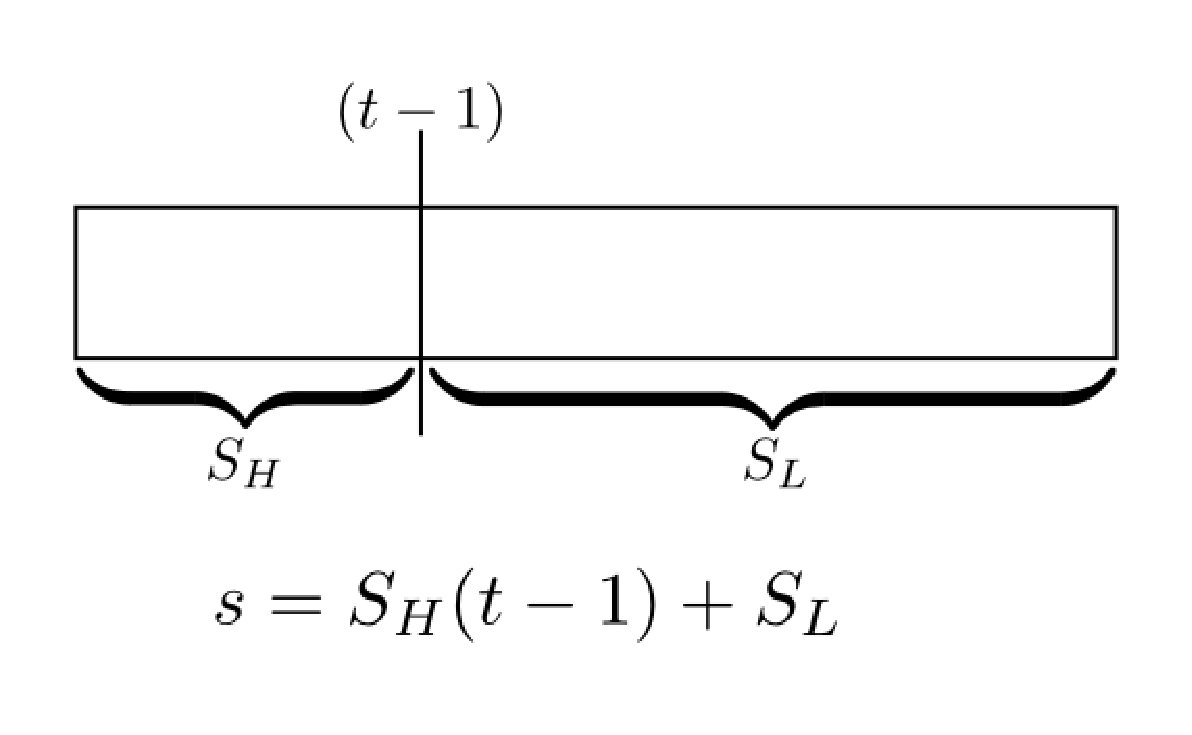
\includegraphics[width=2.5in]{t_adic.eps}
\caption{$(t-1)$ -adic representation of scalar $s$.}
\label{fig:t_adic}
\end{figure}

Figure \ref{fig:z_adicl} shows the final $z$-adic representation of scalar $s$. 
\begin{figure}[!ht]
\centering
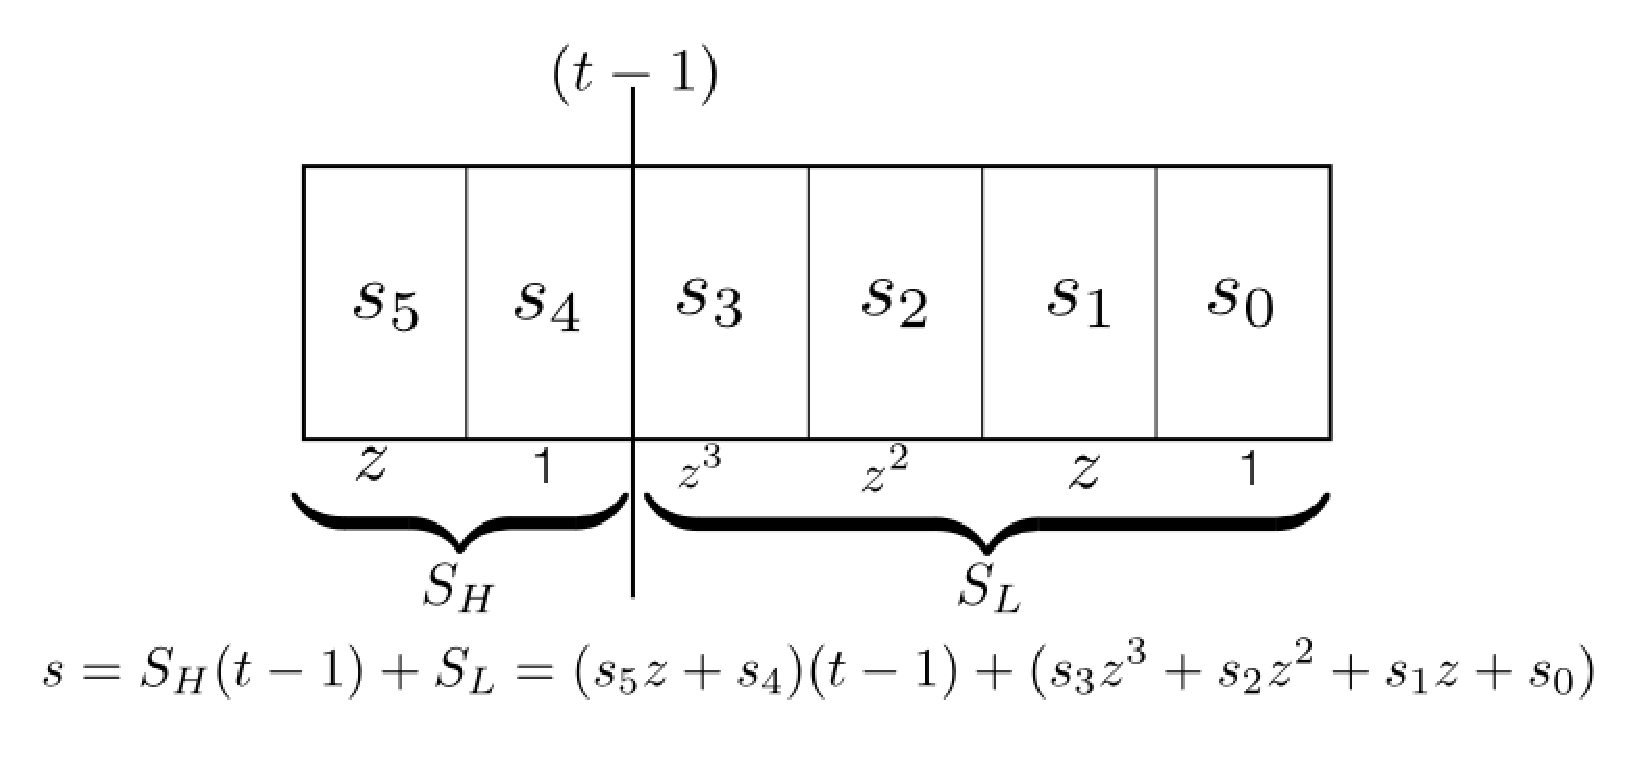
\includegraphics[width=2.5in]{z_adic.eps}
\caption{$z$-adic and $(t-1)$-adic representation of scalar $s$.}
\label{fig:z_adicl}
\end{figure}

Figure \ref{fig:z_sml} shows, an example of multi-scalar multiplication process, implemented in the experiment.
\begin{figure}[!ht]
\centering
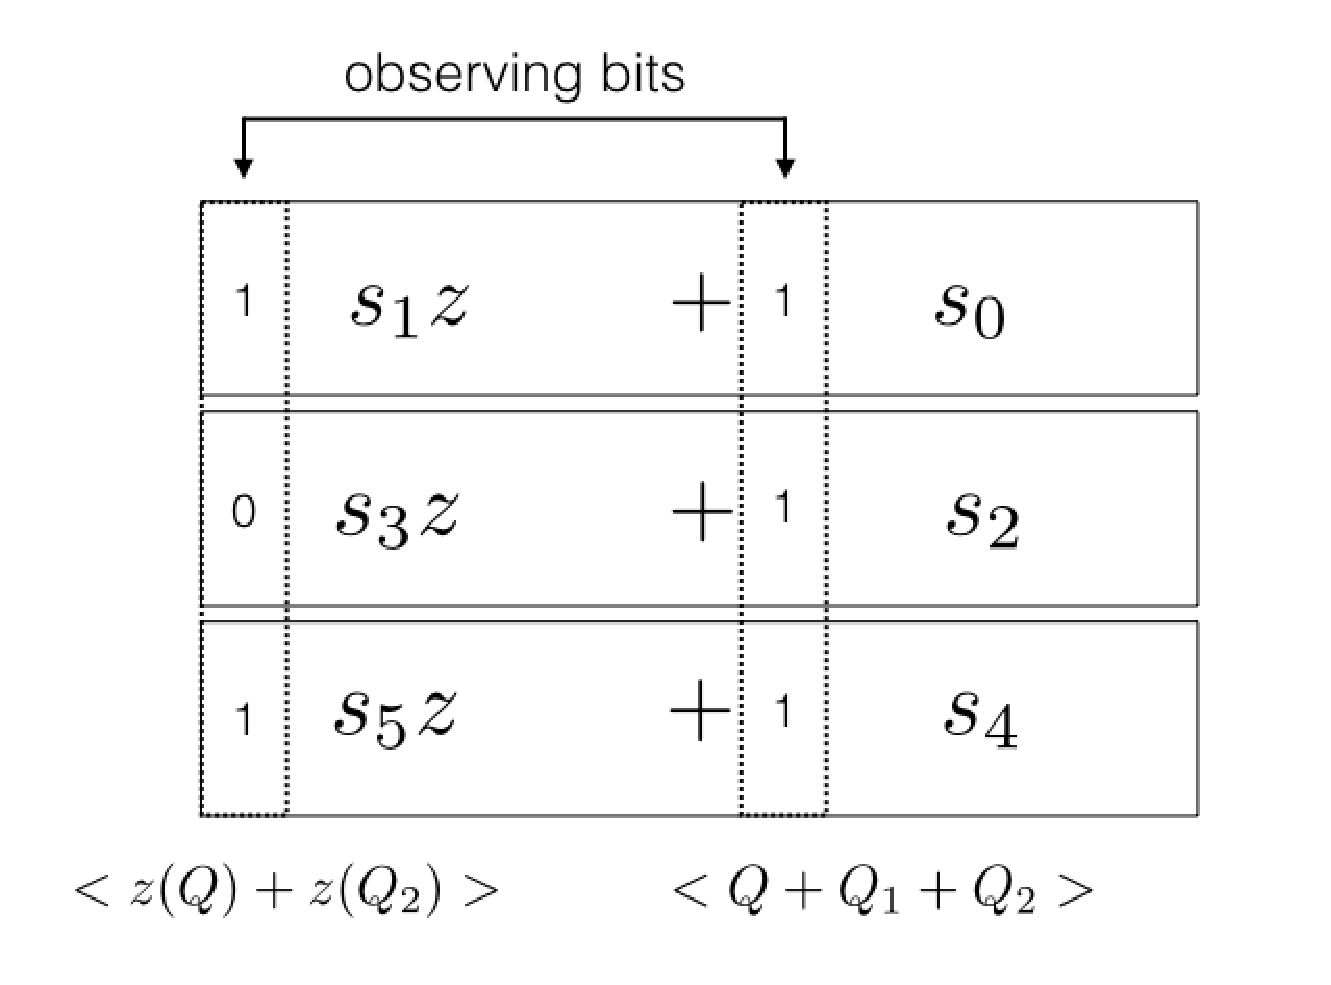
\includegraphics[width=2.5in]{z_sm.eps}
\caption{Multi-scalar multiplication of $s$ with Frobenius mapping.}
\label{fig:z_sml}
\end{figure}

\subsubsection{\g1, \g2 and \g3 groups.} In the context of pairing-based cryptography, especially on KSS curve, three groups $\g1, \g2$, and $\mathbb{G}_3$ are considered. From \cite{mori}, we define $\g1$, $\g2$ and $\g3$ as follows:
\begin{eqnarray}\label{eq:g1}
\g1 & = &  E(\F{p}{k}) [r] \cap \text{Ker}(\pi_p - [1]), \nonumber \\
\g2 & = &  E(\F{p}{k}) [r] \cap \text{Ker}(\pi_p - [p]), \nonumber \\
\g3 & = & \mF{p}{k}/(\mF{p}{k})^r, \nonumber
\end{eqnarray}
\begin{equation}
\alpha : \g1 \times \g2 \rightarrow \g3,
\end{equation}
where $\alpha$ denotes Ate pairing. In the case of KSS curve, $\g1, \g2$ are rational point groups and $\mathbb{G}_3$ is the multiplicative group in $\FQEN$. They have the same order $r$. 

Let us consider a rational point $Q\in \g2 \subset E(\F{p}{18})$.
In the case of KSS curve, it is known that $Q$ satisfies the following relations,
\begin{eqnarray}\label{eq:Q_rel1}
\big[p+1-t\big]Q & = & \cal O, \nonumber \\
\big[t-1\big]Q  & = & \big[p\big]Q.
\end{eqnarray}
\begin{eqnarray}\label{eq:Q_rel2}
[\pi_p -p]Q & = &\cal O, \nonumber \\
\pi_p(Q) & = & [p]Q.
\end{eqnarray}
Thus, these relations can accelerate a scalar multiplication in $\g2$.
Substituting $[p]Q$ in \eqref{eq:Q_rel1} we find $[t-1]Q = \pi_p(Q)$.

\subsubsection{$z$-adic representation of scalar $s$.}
From the previous work on optimal-ate pairing, Aranha et al. \cite{PAIRING:AFKMR12} derived the following relation from parameters \eqref{eq:kss_char}, \eqref{eq:kss_degree}, \eqref{eq:kss_trace} of KSS curve.
\begin{equation}\label{eq:aranha_relation}
z+3p-p^4 \equiv 0 \bmod {r}.
\end{equation}
Here $z$ is the mother parameter of KSS curve and $z$ is about six times smaller than the size of order $r$. 

Let us consider scalar multiplication $[s]Q$, where $0 \leq s < r$. From \eqref{eq:kss_degree} we know $r$ is the order of KSS curve  where $[r]Q=\cal O$. Here, the bit size of $s$ is nearly equal to $r$. In KSS curve $t$ is  $4/6$ times of  $r$. Therefore, let us first consider $(t-1)$-adic representation of $s$ as follows:
\begin{equation}\label{eq:t-1_adic}
s =  S_H(t-1)+S_L,
\end{equation}
where $s$ will be separated into two coefficients $S_H$ and $S_L$.  Size of $S_L$ will be nearly equal to the size of $(t-1)$ and $S_H$ will be about half of $(t-1)$. 
Now we consider $z$-adic representation of $S_H$ and $S_L$ as follows:
%Then SM  $[s]Q$ is calculated as follows:
\begin{eqnarray}\label{eq:scalar_mul_Q}
S_H & =  & s_5+ s_4,\nonumber \\
S_L & = & s_3 z^3+s_2 z^2+s_1 z+s_0.\nonumber 
\end{eqnarray}
Finally $s$ can be represented as 6 coefficients as follows:
\begin{eqnarray}\label{eq:sclar_final_rep}
s & =  & \sum_{i=0}^{3} s_iz^i + (s_4+s_5z)(t-1),\nonumber \\
s & = & (s_0+s_1z) + (s_2 +s_3z)z^2 +(s_4+s_5z)(t-1).
\end{eqnarray}

\subsubsection{Reducing the number of ECA and ECD for calculating $[s]Q$.}
Let us consider a scalar multiplication of $Q \in \g2$ in \eqref{eq:sclar_final_rep} as follows:
\begin{equation}\label{eq:proposed_scm_1}
[s]Q =  (s_0+s_1z)Q + (s_2 +s_3z)z^2Q +(s_4+s_5z)(t-1)Q.
\end{equation}
Let us denote $z^2Q$, $(t-1)Q$ of \eqref{eq:proposed_scm_1} as $Q_1$ and $Q_2$ respectively. From \eqref{eq:aranha_relation} and \eqref{eq:Q_rel2} we can derive the $Q_1$ as follows:
\begin{eqnarray}\label{eq:Q1}
Q_1& = & z^2 Q, \nonumber \\
& = & (9p^2-6p^5+p^8)Q,\nonumber \\
& = & 9\pi^2(Q)-6\pi^5(Q)+\pi^8(Q).
\end{eqnarray}
Using the properties of cyclotomic polynomial \eqref{eq:Q1} is simplified as,
\begin{eqnarray}\label{eq:Q1.1}
Q_1 & = & 8\pi^2(Q)-5\pi^5(Q),  \nonumber\\
& = & \pi^2(8Q)-\pi^5(5Q). 
\end{eqnarray}
And from the \eqref{eq:Q_rel1} and \eqref{eq:Q_rel2}, $Q_2$ is derived as,
\begin{equation}\label{eq:proposed_scm_2}
Q_2 = \pi (Q).
\end{equation}

Substituting \eqref{eq:Q1.1} and \eqref{eq:proposed_scm_2} in \eqref{eq:proposed_scm_1}, the following relation is obtained. 
\begin{equation}\label{eq:proposed_scm_0}
s[Q] =  (s_0+s_1z)Q + (s_2 +s_3z)Q_1 +(s_4+s_5z)Q_2.
\end{equation}
Using $z \equiv -3p + p^4$ (mod $r$) from \eqref{eq:aranha_relation}, $z(Q)$ can be pre-computed as follows:
\begin{equation}
z(Q) = \pi(-3Q) +\pi^4(Q).
\end{equation}
Table \ref{pre-compute} shows all the pre-computed values of rational points for the proposed method. In this paper pre-computed rational points are denoted such as $<Q+Q_2>$. Finally applying the the multi-scalar multiplication technique in \eqref{eq:proposed_scm_0} we can efficiently calculate the scalar multiplication. Figure \ref{fig:z_sml} shows an example of this multiplication. Suppose in an arbitrary index, from left to right, bit pattern of $s_1$, $s_3$, $s_5$ is 101 and at the same index $s_0$, $s_2$, $s_4$ is 111. Therefore we apply the pre-computed points $< z(Q)+z(Q_2) >$ and $<Q+Q_1+Q_2>$ as ECA in parallel. Then we perform ECD and move to the right next bit index to repeat the process until maximum length $z$-adic coefficient becomes zero.

\renewcommand{\baselinestretch}{1.5}
\begin{table}[!ht]
\centering
\caption{ Pre-computed values of rational point for efficient scalar multiplication}
\label{pre-compute}
\begin{tabular}{|c|c|}
\hline 
• & $z(Q)$ \\ 
\hline 
$Q_1$ & $z(Q_1)$  \\ 
\hline 
$Q_2$ & $z(Q_2)$ \\ 
\hline 
$Q_1+Q_2$ & \quad  $ z(Q_1)+ z(Q_2) $ \quad \\ 
\hline 
$Q+Q_2$ & $ z(Q)+ z(Q_2) $ \\ 
\hline 
$Q+Q_1$ & $  z(Q)+ z(Q_1) $ \\ 
\hline 
 \quad $Q+Q_1+Q_2$ \quad  \quad &   \quad  $ z(Q)+ z(Q_1)+ z(Q_2)$  \quad \\ 
\hline 
\end{tabular} 
\end{table}
\renewcommand{\baselinestretch}{1.0}
As shown in Figure \ref{fig:z_sml}, during scalar multiplication in parallel, we are considering \eqref{eq:sclar_final_rep} like 3 pair of coefficients of $z$-adic representation. If we consider 6-coefficients for parallelization, we will need to calculate $2^6 \times 2$ pre-computed points. The chance of appearing each pre-computed point in parallel calculation will be only once which will make the pre-calculated points redundant.  

\section{Experimental result evaluation}
In order to demonstrate the efficiency of the proposal, this section shows some experimental result with the calculation cost. In the experiment we have compared the proposed method with three well studied method of scalar multiplication named binary method, sliding-window method and non-adjacent form (NAF) method.

In the experiment the following parameters are considered for the KSS curve $y^2 = x^3 + 11$. 
\begin{eqnarray}
z & = & 65   \mbox{-bit},  \nonumber \\ 
p  & = & 511 \mbox{-bit},  \nonumber \\ 
r  & = & 378 \mbox{-bit} ,\nonumber \\ 
t  & = & 255  \mbox{-bit}. \nonumber
\end{eqnarray}
The mother parameter $z$ is also selected accordingly to find out $\g2$ rational point $Q$. 

500 scalar numbers of size (about 377-bit) less than order $r$ is generated randomly in the experiment. Then average number of ECA and ECD for the proposed method and the three other methods is calculated for a scalar multiplication. 13  pre-computed ECA is taken into account while the average is calculated for the proposed method. In case of sliding-window method window size 4-bit is considered. Therefore 14 pre-computed ECA is required. In addition, average execution time of the proposed method and the three other methods is also compared.

Table \ref{tab1} shows the environment, used to experiment and evaluate the proposed method.  
\renewcommand{\baselinestretch}{1.5}
\begin{table}[!ht]
\renewcommand{\arraystretch}{1.3}
\centering
\caption{ Computational Environment}
\label{tab1}
\begin{tabular}{|c|c|c|}
\hline 
• & PC & iPhone6s \\ 
\hline \hline 
CPU {\textsuperscript{*}} & \quad 2.7 GHz Intel Core i5 \quad & \quad Apple A9 Dual-core 1.84 GHz \quad \\ 
\hline 
Memory & 16 GB & 2 GB \\ 
\hline 
OS & Mac OS X 10.11.4 &  iOS 9.3.1 \\ 
\hline 
Compiler & gcc 4.2.1 & gcc 4.2.1 \\ 
\hline 
\quad Programming Language \quad  & C & Objective-C, C \\ 
\hline 
Library & GNU MP 6.1.0 & GNU MP 6.1.0 \\ 
\hline 
\midrule[.5pt]
\multicolumn{3}{l}{\textsuperscript{*}\footnotesize{Only single core is used from two cores.}}\\
\end{tabular} 
\end{table}
\renewcommand{\baselinestretch}{1.0}

\renewcommand{\baselinestretch}{1.5}
\begin{table}[!ht]
%\renewcommand{\arraystretch}{1.3}
\centering
\caption{ Comparative result of average number of ECA and ECD and execution time in [ms] for scalar multiplication}
\label{tab_opeation}
\begin{tabular}{|c|c|c|c|c|c|c|}
\hline
 & \multicolumn{6}{|c|}{\quad Average ECA, ECD and  execution time [ms] comparison \quad} \\ \hline
& \multicolumn{2}{|c|}{PC} & PC & \multicolumn{3}{|c|}{iPhone 6s}  \\ 
 \hline \hline
Methods & \quad \#ECA \quad & \quad \#ECD \quad & \quad Execution time \quad & \multicolumn{3}{|c|}{\quad Execution time}\\ 
 \hline
Binary  & 187 & 376 &  $1.15 \times 10^3$  &  \multicolumn{3}{|c|} { $1.3 \times 10^3$}\\ \hline
\quad Sliding-window \quad & 103 & 376 &  $1.14 \times 10^3$  &  \multicolumn{3}{|c|} { $1.10 \times 10^3$}\\ \hline
 NAF  & 126 & 377 &  $1.03 \times 10^3$  &  \multicolumn{3}{|c|} { $1.13 \times 10^3$}\\ \hline
 \quad Proposed  \quad \quad & 124 & 64 & $3.36 \times 10^2$  &   \multicolumn{3}{|c|}{$3.76 \times 10^2$}\\ \hline
\end{tabular} 
\end{table}
\renewcommand{\baselinestretch}{1.0}
Analyzing  Table \ref{tab_opeation} we can find that our proposed method requires more than 5 times less ECD than binary method, sliding-window method and NAF method. The number of ECA is also reduced in the proposed method by about 30\% than binary method.  

In this experiment, execution time may seems slower than other efficient algorithm such as Montgomery reduction. 
But the main purpose of this execution time comparison is to compare the ratio of the execution time of the proposed method with other well studied methods. The result shows that proposed method is at least 3 times faster than the other methods. Other acceleration techniques such as Montgomery reduction, Montgomery trick and efficient coordinates can be applied to this proposed method to enhance its execution time.

\section{Conclusion and future work}
In this paper we have proposed an efficient method to calculate elliptic curve scalar multiplication using Frobenious mapping  over KSS curve in context of pairing based cryptography. We have also applied $(t-1)$-adic and $z$-adic representation on the scalar and have applied multi-scalar multiplication technique to  calculate scalar multiplication in parallel. We have evaluated and analyzed the improvement by implementing a simulation for large size of scalar in 192-bit security level. The experimented result shows that our proposed method is at least 3 times efficient in context of execution time and takes 5 times less number of elliptic curve doubling than binary method, sliding-window method and non-adjacent form method. As a future work we would like to enhance its computation time by applying not only Montgomery reduction but also skew Frobenius  map in  sub-field isomorphic rational point group technique and test the effect of the improvement in some pairing application for practical case. 

\section*{Acknowledgment}
This work was partially supported by the Strategic Information and Communications R\&D Promotion Programme (SCOPE) of Ministry of Internal Affairs and Communications, Japan. 

%\medskip
%\bibliographystyle{1}
%\bibliography{wisa_ref.bib}

% \end{document}